\chapter{Theoretischer Teil}
\label{chapter_TheoretischerTeil}
Dieses Kapitel befasst sich mit den theoretischen Grundlagen, die für den Einsatz von \acp{SBC} zur Datenerfassung mittels verschiedener Sensoren nötig sind. In Abschnitt \ref{section_Begriffsdefiniton} werden die im weiteren Verlauf der Arbeit verwendeten Fachbegriffe erläutert, um die beschriebenen Zusammenhänge gut zu verstehen. Der Abschnitt \ref{section_Vergleich_SBC} behandelt die unterschiedlichen sich auf dem Markt befindenden \acp{SBC} mit ihren jeweiligen Vor- bzw. Nachteilen. Die verschiedenen Bussysteme wie z.B. der \ac{I$^2$C}  Bus werden in Abschnitt \ref{section_Bussysteme} erklärt und deren Funktionsweise erläutert. 


\section{Begriffsdefinitionen}
\label{section_Begriffsdefiniton}
Die in diesem Abschnitt beschriebenen Definitionen wurden, soweit nicht anders angegeben aus folgendem Dokument entnommen \citep{Bussysteme_in_der_Praxis}.

\subsection*{Single Board Computer}
Unter einem \textit{Single Board Computer} (\ac{SBC}) versteht man ein Computersystem, welches sich komplett auf einer einzigen Platine befindet. \acp{SBC} können fast die gleichen Aufgaben erledigen wie gewöhnliche Computer, allerdings sind die Einplatinen-Rechner diesen im Hinblick auf die Hardwareausstattung (z.B. Größe des Speichers, Taktfrequenz der CPU etc.) um einiges unterlegen.

\subsection*{Bussysteme}
\textit{Bussysteme} sind Systeme, die  zur seriellen Datenübertragung zwischen einen oder mehreren Komponenten verwendet werden. Beispiele hierfür sind der \ac{I$^2$C} Bus, der \ac{SPI} Bus oder auch der \ac{CAN} Bus. Eine genauere Beschreibung der Bussysteme folgt in Abschnitt \ref{section_Bussysteme}.

\subsection*{Raspberry Pi}
Der \textit{\ac{RPI}} ist ein \ac{SBC}, der von der britischen \textit{Raspberry Pi Foundation} aus Komponenten von Android-Smartphones entwickelt wurde.

\subsection*{Raspbian}
\textit{Raspbian} ist ein Betriebssystem, welches auf der Linux Distribution Debian basiert und speziell auf den Raspberry Pi angepasst wurde.

\subsection*{RRDTool}
Das \textit{RRDTool} ist ein Programm, mit dem man Round-Robin Datenbanken erstellen kann. Diese Datenbanken eignen sich besonders gut für die Aufzeichnung von zeitlich fortlaufenden Datenreihen wie z.B. Temperatur- oder Strommessungen. Die Datenbank liegt dabei in einem einzigen File auf dem Datenträger und hat ab dem Erstellen eine feste Größe, die sich auch bei vielen Messungen über einen längeren Zeitraum nicht vergrößert. 

\subsection*{General Purpose Input/Output}
\textit{\ac{GPIO}} sind elektrische Kontakte auf einem SBC, die zur Realisierung verschiedener Funktionen für elektronische Geräte verwendet werden \citep{Raspberri_Pi_Handbuch}. Eine genauere Erklärung erfolgt in Abschnitt \ref{subsection_GPIO} .

\subsection*{Python}
\textit{Python} ist eine Programmiersprache, die vor allem auf dem Raspberry Pi bevorzugt verwendet wird.

\subsection*{Bluetooth Low Energy}
\textit{\ac{BLE}} ist eine Funktechnologie, die es ermöglicht, dass sich Geräte in unmittelbarer Entfernung zueinander vernetzen lassen. Der Strombedarf bei \ac{BLE} ist um einiges geringer als bei herkömmlichen Bluetooth \citep{Bluetooth_Low_Energy}.
\subsection*{Windows 10 IoT}
\textit{Windows 10 IoT} ist eine \glqq abgespeckte\grqq \;Version von Windows 10, die auf mobilen Geräten wie dem Raspberry Pi\,3 lauffähig ist. IoT steht dabei für \textit{Internet of Things} \citep{Raspberri_Pi_Handbuch}.

%Abschnitt Vergleich von SBCs 
\section{Vergleich von verschiedenen SBCs}
\label{section_Vergleich_SBC}
In diesem Abschnitt werden einige der bekanntesten \acp{SBC}, die sich auf dem Markt befinden, miteinander verglichen, um den bestmöglichen für die vorgegebenen Anforderungen auswählen zu können.
Wichtige Kriterien für die Auswahl sind, dass die Möglichkeit besteht, verschiedene Betriebssysteme (Windows und Linux) mit dem jeweiligen Einplatinenrechner betreiben zu können. Vergleichskriterium ist die Unterstützung von verschiedenen Kommunikationsschnittstellen (\ac{I$^2$C}, \ac{SPI}, 1-Wire), um eine große Anzahl von Sensoren nutzen zu können. Eine Übersicht der verschiedenen \acp{SBC} ist in den Tabellen \ref{Tabelle_Vergleich_SBC1} und \ref{Tabelle_Vergleich_SBC2} dargestellt.

%Tabelle 1
\begin{table}[H]
%\rowcolors{2}{black!10}{black!20}
\centering
\begin{tabular}{
llll
}
\toprule
\multicolumn{1}{p{3cm}}{\textit{\ac{SBC}}} & \multicolumn{1}{p{3.5cm}}{\textit{Operating System} } & \multicolumn{1}{p{1,5cm}}{\textit{RAM} }&\multicolumn{1}{p{3cm}}{ \centering\textit{CPU} }\\\midrule
Banana Pi & Linux, Android & 1 GB & ARM Cortex-A7, 1 GHz\\
&&&\\
Raspberry Pi3&Windows, Linux&1 GB&ARM Cortex-A53 1,2 GHz\\
&&&\\
BeagleBone Black & Linux & 512 MB & ARM Cortex-A8 1 GHz\\
&&&\\
HummingBoard i2eX & Linux, Android & 1 GB & ARM Cortex-A9 1 GHz\\
&&&\\
Intel Galileo Gen 2 & Windows, Linux & 256 MB & x86 Quark 400 MHz\\
&&&\\
Radxa Rock & Linux & 2 GB & ARM Cortex-A9 1,6 GHz\\
\bottomrule
\end{tabular}
\caption{Vergleich OS, RAM, CPU verschiedener SBCs \citep{Quelle_Tabelle} \citep{RaspberryPiHomePage}}
\label{Tabelle_Vergleich_SBC1}
\end{table}

\begin{threeparttable}[H]
%\rowcolors{2}{black!10}{black!20}
\centering
\begin{tabular}{
llll
}
\toprule
\multicolumn{1}{p{3cm}}{\textit{\ac{SBC}}} & \multicolumn{1}{p{3.5cm}}{\textit{Communication} } & \multicolumn{1}{p{3cm}}{\textit{Networking} }&\multicolumn{1}{p{3cm}}{ \textit{GPIO} }\\\midrule
Banana Pi & I$^2$C, SPI & 1\;GigE & 80\\
&&&\\
Raspberry Pi3&I$^2$C, SPI&10/100\;Mbps\tnote{1} &40\\
&&&\\
BeagleBone Black &I$^2$C, SPI&10/100\;Mbps&66\\
&&&\\
HummingBoard i2eX &I$^2$C, SPI&1\;GigE&8\\
&&&\\
Intel Galileo Gen 2 & I$^2$C, SPI&10/100\;Mbps&20\\
&&&\\
Radxa Rock & I$^2$C, SPI\tnote{2}&10/100\;Mbps&80\\
\bottomrule
\end{tabular}

\begin{tablenotes}\footnotesize
\item[1] mit WLAN on Board
\item[2] nur für Android
\end{tablenotes}

\caption{Vergleich Schnittstellen, Netzwerkverbindung, Anzahl GPIO Pins \citep{Quelle_Tabelle} \citep{RaspberryPiHomePage}}
\label{Tabelle_Vergleich_SBC2}
\end{threeparttable}

Wie aus den Tabellen ersichtlich ist, unterstützen die meisten aktuellen \acp{SBC} das Betriebssystem Linux. Eine Anforderung für diese Projekt war allerdings, dass sowohl ein Linux System, wie auch ein Windows System auf dem Board lauffähig ist, um sich im späteren Verlauf des Projektes nicht auf ein Betriebssystem einzuschränken. Aus diesem Grund fiel die Wahl auf den \ac{RPI}\;3, da dieser beide Betriebssysteme unterstützt und auch bei den anderen betrachteten Aspekten wie \textit{RAM, CPU} etc. den meisten Boards ebenbürtig oder sogar überlegen ist. Ein weiterer wichtiger Entscheidungsgrund für den \ac{RPI}\;3 war, dass es für diesen eine sehr große Anzahl an unterstützten Sensoren gibt (Sensoren die mit einer elektrischen Spannung von 3,3\;$V$ - 5\;$V$ betrieben werden). Dies ermöglicht einen sehr weit gefächerten Einsatz des \ac{RPI}\;3, was für das vorgesehene Projekt von großer Bedeutung ist.

%%Kapitel Raspberry PI
\section{Raspberry Pi 3}
\label{section_Raspberry_Pi3}
Das folgende Kapitel beschreibt den Raspberry Pi 3 und befasst sich genauer mit den verbauten Komponenten, welche im weiteren Verlauf der Arbeit benötigt werden. 

\subsection{Allgemeine technische Daten}
\label{subsection_Allgemeine_technische_Daten}
Die folgenden Information wurden, soweit nicht anders angegeben von der offiziellen Homepage der \textbf{Raspberry Pi Foundation} entnommen \citep{RaspberryPiHomePage}.\\
Der \ac{RPI}\;3 ist ein kreditkartengroßer Einplatinenrechner, welcher aktuell an die \textit{sieben Million} Mal verkauft wurde \citep{RPI_Verkaufszahlen}. Dieser besitzt:
\begin{itemize}
\item einen 1.2\;GHz 64-bit quad-core ARMv8 CPU
\item 802.11n Wireless LAN
\item Bluetooth 4.1
\item \ac{BLE}
\item 4 USB Ports
\item 40 GPIO Pins
\item Full HDMI Port
\item Ethernet Port
\item \ac{CSI}
\item \ac{DSI}
\item Micro SD Karten Slot
\end{itemize}

Die aktuelle Version des Raspberry Pi, der \ac{RPI}\;3 ist in Abbildung \ref{Abb_Bild_RPI3} dargestellt.

\begin{figure}[!h] 
  \centering
     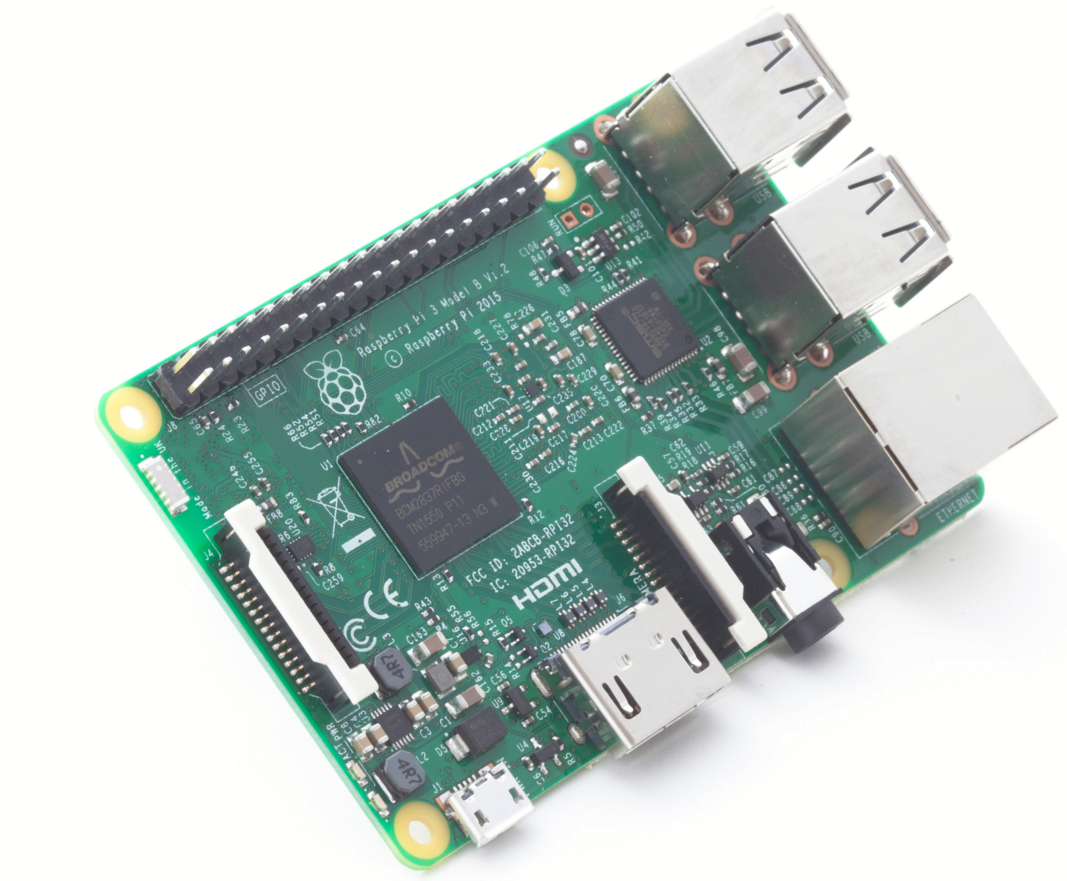
\includegraphics[scale=.4]{BilderAllgemein/RPI3.png}
  \caption{Raspberry Pi\;3 \citep{RPI_Bild}}
  \label{Abb_Bild_RPI3}
\end{figure}

Durch die im Gegensatz zu den Vorgänger Modellen leistungsstärkere CPU mit einem 64-Bit quad-core Prozessor, ist es beim RPI\;3 möglich das Windows Betriebssystem \textit{Windows 10 IoT} zu betreiben, wodurch sich eine Erweiterung der Einsatzmöglichkeiten ergibt. Auch wurde im Gegensatz zu den vorherigen Modellen  ein WLAN Modul (2,4\;GHz) gleich auf der Platine verbaut und muss nicht mehr durch ein externes USB-WLAN Modul realisiert werden. Der \ac{RPI}\;3 bietet weiterhin einen 10/100 MBit Ethernet Anschluss sowie einen \ac{CSI} und \ac{DSI} Anschluss zur direkten Anbindung einer Kamera oder Displays. Die verschiedenen GPIO-Pins werden in Kapitel \ref{subsection_GPIO} genauer beschrieben.

\subsection{GPIO-Kontakte}
\label{subsection_GPIO}
Im Gegensatz zu den Vorgängermodellen des \ac{RPI}\;3, welche nur 26 GPIO Pins besaßen, besitzt der \ac{RPI}\;3 40 GPIO Pins. Diese sind in Abbildung \ref{Abb_Bild_RPI3} ersichtlich am linken oberen Ende der Platine zu 2\;x\;20 Kontakten angeordnet. Der Rasterabstand von einem Pin zum nächsten beträgt 2,54 mm. Die GPIO-Pins sind elektrische Kontakte, die zur Messung und Steuerung von elektronischen Geräten wie z.B. Sensoren, Analog Digital Wandlern, LEDs etc. verwendet werden.\\
Die Steckerleiste beinhaltet einige allgemein verwendbare Pins (\textit{=\;General Purpose Input\;/\;Output}), sowie zwei verschiedene Spannungsversorgungen (\textit{3,3\;V} und \textit{5\;V}) und Masse Anschlüsse (\textit{0\;V}). Weiterhin beinhaltet die Steckerleiste Kontakte für den \ac{I$^2$C}-, \ac{SPI}- und 1-Wire-Bus. Bei der Verwendung der GPIO-Kontakten für verschiedene Projekte muss darauf geachtet werden, welche Bezeichnung verwendet wird. Die drei Möglichkeiten sind:
\begin{itemize}
\item die physikalische Pin-Nummer, anhand seine Position auf dem Board (von oben gesehen, Pin 1 besitzt eine quadratische Lötstelle)
\item die BCM-Pin-Nummer, welche sich auf die Nummerierung der offiziellen Dokumentation des BCM2836-Chips bezieht
\item den Pin Namen, welcher von den \ac{RPI} Entwicklern vergeben wurde 
\end{itemize} 
vorgenommen werden \citep{Raspberri_Pi_Handbuch}.\\\\
In Abbildung \ref{Abb_Bild_GPIO} ist die Pin Belegung des \ac{RPI}\;3 grafisch dargestellt.

%Grafik GPIO Pins
\begin{figure}[!h] 
  \centering
     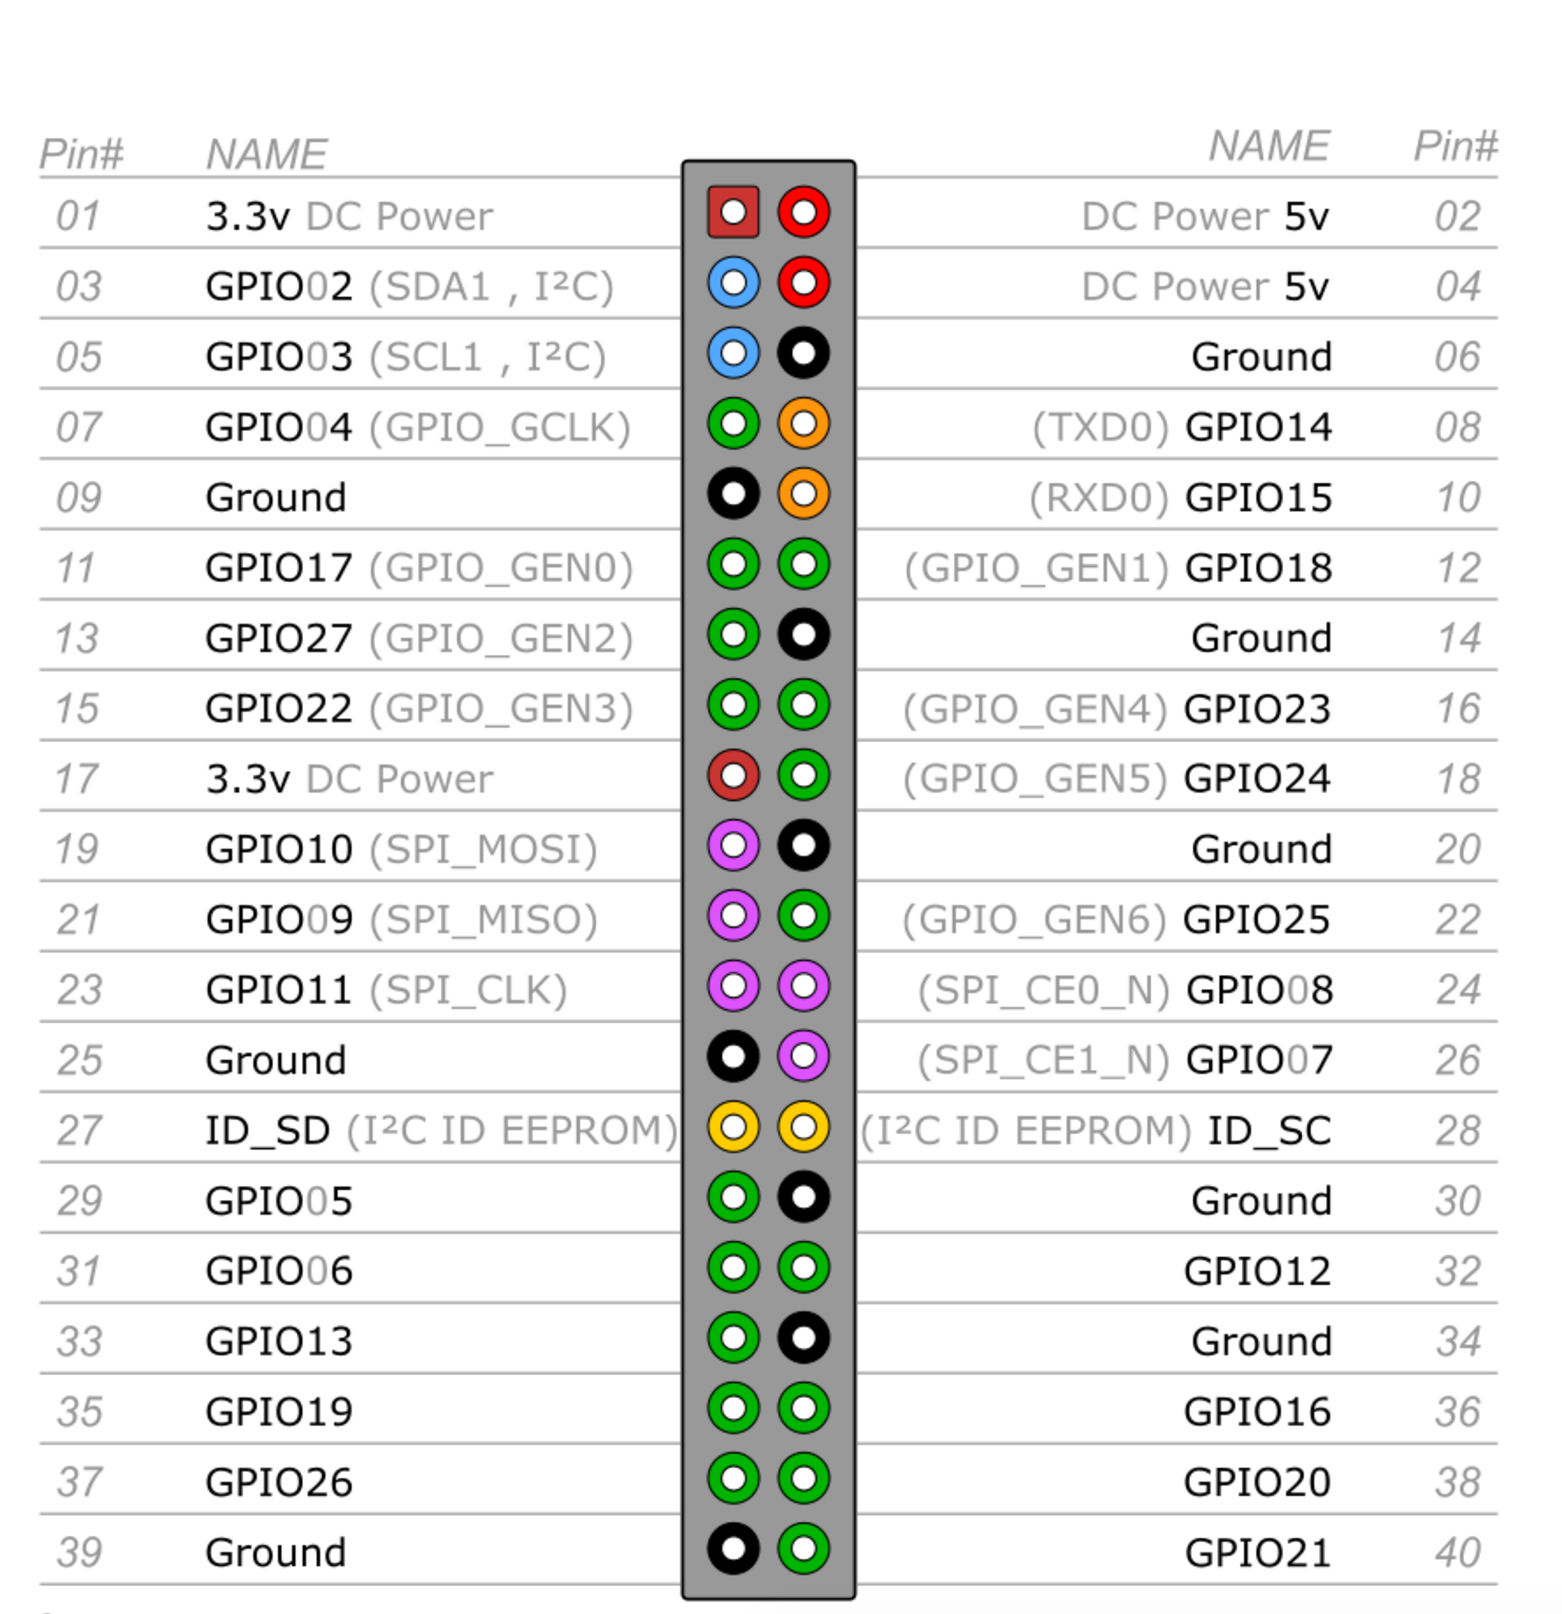
\includegraphics[scale=.35]{BilderAllgemein/GPIO.png}
  \caption{GPIO-Kontakte \citep{GPIO_Header_Bild}}
  \label{Abb_Bild_GPIO}
\end{figure}

%% Section Bussysteme
\section{Bussysteme}
\label{section_Bussysteme}
Im folgenden Kapitel werden die am häufigsten verwendeten Bussysteme für die verschiedenen Sensoren erläutert. Zu diesen Bussystemen gehören der \textit{1-Wire}, \textit{\ac{I$^2$C}} und der \textit{\ac{SPI}} Bus. 

\subsection{1-Wire}
\label{subsection_1Wire}
Der 1-Wire Bus ist ein serielles Bussystem von der Firma \textit{Dallas\footnote{2001 von Maxim Integrated übernommen}} , bei dem die Daten seriell (nacheinander) über eine Datenleitung übertragen werden.
\subsubsection*{Allgemeine Informationen}
\label{subsection_Allgemeine_Informationen_1Wire}
 Für dieses Bussystem wird nur eine Datenleitung benötigt, die auch als Spannungsversorgung für den\;/\;die jeweiligen Sensoren benutzt wird. Physikalisch werden allerdings zwei Leitungen verwendet, da die Masse auch mitgeführt werden muss. Es gibt für diesen Bus eine große Anzahl an Sensoren wie z.B. Temperatursensoren, die sich durch einen sehr geringen Stromverbrauch auszeichnen. Während der Kommunikation wird der Sensor aus einem internen Kondensator gespeist. Allerdings kann es notwendig sein, bei Sensoren bei denen die interne Spannungsversorgung nicht ausreichend ist, eine extra Spannungsversorgung für den jeweiligen Sensor mitzuführen. \\
Der 1-Wire Bus ist ein \textit{One-Master-Multi-Slave} Bussystem, was bedeutet, dass es  einen Master (z.B. \ac{RPI}\;3) und mehrere Slaves (z.B. Sensoren) gibt. Die Aufgabe des Masters  ist es, die Kommunikation zu steuern. Die maximale Anzahl der Sensoren kann bis zu 100 betragen, welche parallel zueinander an den Master angeschlossen werden. Dies ist möglich, da jeder Sensor ein eindeutige 64 Bit lange ID besitzt \citep{Bussysteme_in_der_Praxis}.


\subsubsection*{Übertragungsprotokoll}
\label{subsection_Protokoll_1Wire}
Der 1-Wire Bus wird dadurch, dass er kein Taktsignal benötigt, als \textit{asynchroner} Bus bezeichnet. Dieser kommuniziert im \textit{Halbduplex} Verfahren, was bedeutet, dass immer nur ein Teilnehmer auf dem Bus senden oder empfangen kann (entweder Master oder ein Slave). Wenn keine Kommunikation stattfindet, wird die Datenleitung über einen Pullup-Widerstand auf \textit{high} gezogen\footnote{bedeutet, dass durch den Pullup Widerstand exakt die Versorgungsspannung z.B. 3,3\,V anliegt} und der zuvor erwähnte interne Kondensator geladen.  Wenn eine Übertragung stattfindet liegt die Datenleitung auf Masse und der Kondensator liefert in diesem Fall die Spannungsversorgung für den Sensor (abhängig vom Sensor). Dadurch, dass keine Taktleitung vorhanden ist, muss für die Kommunikation ein bestimmter Ablauf eingehalten werden (siehe Tabelle \ref{Tabelle_Befehle_1Wire}).\\
Die Zeitspanne für die Übertragung von 1 Bit beträgt immer 60\,$\mu s$. Diese Steuerung, egal in welche Richtung die Übertragung stattfindet werden durch den Master initiiert. Die Befehle die dazu notwendig sind, können aus der Tabelle \ref{Tabelle_Befehle_1Wire} entnommen werden \citep{Bussysteme_in_der_Praxis}.

%Tabelle 1
\begin{threeparttable}[H]
%\rowcolors{2}{black!10}{black!20}
\centering
\begin{tabular}{
llll
}
\toprule
\multicolumn{1}{p{2cm}}{\textit{Befehl} }&\multicolumn{1}{p{10cm}}{\centering\textit{Beschreibung} }\\\midrule
\textbf{Write 1} & Der Master zieht für $1-15\;\mu s$ auf Low. Der Rest des Slots bleibt \\
& ungenutzt.\\
&\\
\textbf{Write 0} & Der Master zieht den Bus für mindestens $60\;\mu s$ bis maximal\\
& $120\;\mu s$ auf Low\tnote{3}.\\
&\\
\textbf{Read}& Der Master zieht für $1-15\;\mu s$ auf Low. Der Slave, der kommunizieren\\
& möchte, hält für eine 0 den Bus weiter auf Low\footnote{Hallo}. Will der Slave eine\\
& 1 senden, gibt er direkt den Bus wieder frei. Wie man leicht erkennt,\\
& ist der Status Write 1 oder Read für den Master gleich. Alleine der \\
& Status des Sensors bestimmt, ob ein Read oder Write 1 ausgeführt wird. \\
&\\
\textbf{Reset /} & Der Master zieht den Bus für min. $480\;\mu s$ auf Low. Wenn ein\\
\textbf{Presence} & Slave am Bus vorhanden ist, zieht er max. $60\;\mu s$ (also einen\\
& Slot) die Leitung auf Low. Somit weiß der Master, dass mindestens\\
& ein Slave angeschlossen ist.\\ 
\bottomrule
\end{tabular}
\begin{tablenotes}\footnotesize
\item[3] auf Low ziehen = es liegen exakt 0\,V an
\end{tablenotes}
\caption{Befehle bei 1-Wire \citep[S. 35]{Bussysteme_in_der_Praxis}}
\label{Tabelle_Befehle_1Wire}
\end{threeparttable}

%I2C Bus
\subsection{I$^2$C-Bus}
\label{subsection_I2C}
Der \ac{I$^2$C} Bus ist auch noch unter einem anderen Namen als \ac{TWI} Bus (z.B. bei Atmel) bekannt. Er wurde 1982 von der Firma Philips Semiconductors\footnote{heute NPX} entwickelt und wird vornehmlich zur internen Kommunikation von Geräten benutzt \citep{Bussysteme_in_der_Praxis}.

\subsubsection*{Allgemeine Informationen}
\label{subsubsection_Allgemeine_Informationen_I2C}
Technisch gesehen sind der \ac{I$^2$C} und \ac{TWI} Bus identisch, die Unterscheidung wird lediglich aus lizenzrechtlichen Gründen getroffen. Bei dem Bus handelt es sich um einen \textit{Master-Slave-Bus}, allerdings ist auch ein \textit{Multi-Master\footnote{es gibt mehr als einen Master}} Betrieb möglich. Der Beginn einer Kommunikation wird immer vom Master initiiert, bei dem angesprochenen Multi-Master Betrieb arbeitet dann der vom Initiator angesprochene Master wie ein Slave. Im Gegensatz zum 1-Wire Bus sind zwei Leitungen zur Datenübertragung notwendig, eine Datenleitung (SDA) und eine Taktleitung (SCL). Da der \ac{I$^2$C} Bus eine Taktleitung besitzt, spricht man hier von einem synchronen seriellen Bussystem. Der Systemtakt wird bei diesem System immer vom Master vorgegeben \citep{Bussysteme_in_der_Praxis}. 

\subsubsection*{Definierte Zustände und Adressierung}
\label{subsubsection_definierte_Zustände_Adressierung}
Bei der Kommunikation mittels \ac{I$^2$C} müssen bestimmte Zustände eingehalten werden um die korrekte Funktion sicherzustellen. Diese werden im Anschluss dargestellt. Für die folgenden Definitionen dient falls nicht anders angegeben folgende Quelle \citep{I2C_Datenblatt}.
\subsubsection*{Gültigkeit Datenbit}
\label{subsubsection_Gültigkeit_Datenbit}
Damit ein Bit auf der Datenleitung als gültig betrachtet wird, darf sich dessen Pegel während der High Phase der Taktleitung nicht ändern. Dieser Zustand ist in Abbildung \ref{Abb_Bild_I2C_data_valid} dargestellt.

%Grafik Data valid
\begin{figure}[!h] 
  \centering
     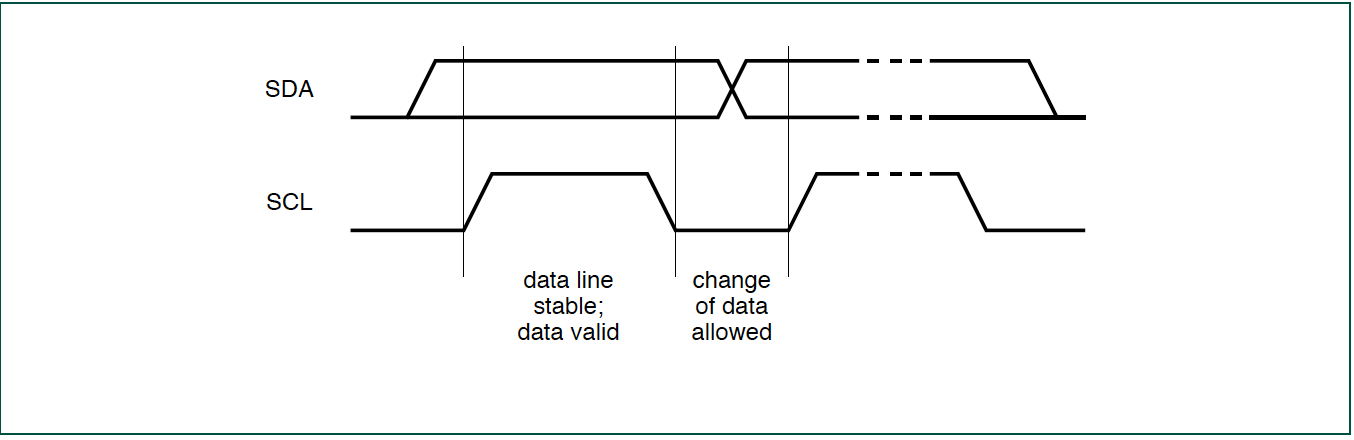
\includegraphics[scale=.65]{BilderAllgemein/I2C_data_valid.png}
  \caption{Bedingung für gültiges Bit auf Datenleitung \citep[S. 9]{I2C_Datenblatt}}
  \label{Abb_Bild_I2C_data_valid}
\end{figure}

\subsubsection*{START Bedingung}
\label{subsubsection_START_Bedingung}
Damit eine Kommunikation stattfinden kann, muss diese als Erstes durch eine Start Bedingung eingeleitet werden.  Realisiert wird die Startbedingung, indem der Master die SDA Leitung auf Ground zieht, während die SCL Leitung auf HIGH gesetzt ist. Abbildung \ref{Abb_Bild_I2C_START_STOP} zeigt diesen Zustand.

\subsubsection*{STOP Bedingung}
\label{subsubsection_STOP_Bedingung}
Um die Übertragung zu beenden, ist die STOP Bedingung definiert. Diese unterscheidet sich von der START Bedingung dadurch, dass der Master bei HIGH Potential der Taktleitung die Datenleitung ebenfalls auf HIGH zieht. Grafisch ist dies in Abbildung \ref{Abb_Bild_I2C_START_STOP} dargestellt.

%Grafik START STOP
\begin{figure}[!h] 
  \centering
     \includegraphics[scale=.65]{BilderAllgemein/I2C_START_STOP.png}
  \caption{START, STOP Bedingung \ac{I$^2$C}  \citep[S. 9]{I2C_Datenblatt}}
  \label{Abb_Bild_I2C_START_STOP}
\end{figure}

% Subsectio Adressierung
\subsubsection*{Adressierung}
\label{subsubsection_Adressierung}
Bei der Adressierung wird nach der Start Bedingung 1 Byte vom Master an den Slave gesendet. Bei diesem Byte stellen die ersten sieben Bits die Adresse des Slaves dar und das achte Bit das Read\,/\,Write Bit. Die Kennzeichnung des R\,/\,W Bits ist immer aus Sicht des Masters zu deuten. Dies bedeutet, dass bei WRITE Daten vom Master an den Slave übertragen werden und bei READ Daten vom Slave an den Master.
Abbildung \ref{Abb_Bild_I2C_Slave_Adresse} verdeutlicht noch einmal den Aufbau des ersten Bytes.\\ Dadurch, dass sieben Bits für die Adresse des Slaves verwendet werden können und 16 Adressen davon für Erweiterungen reserviert sind, können maximal 112 Teilnehmer  an den Bus betrieben werden.


%Grafik Slave Adresse
\begin{figure}[!h] 
  \centering
     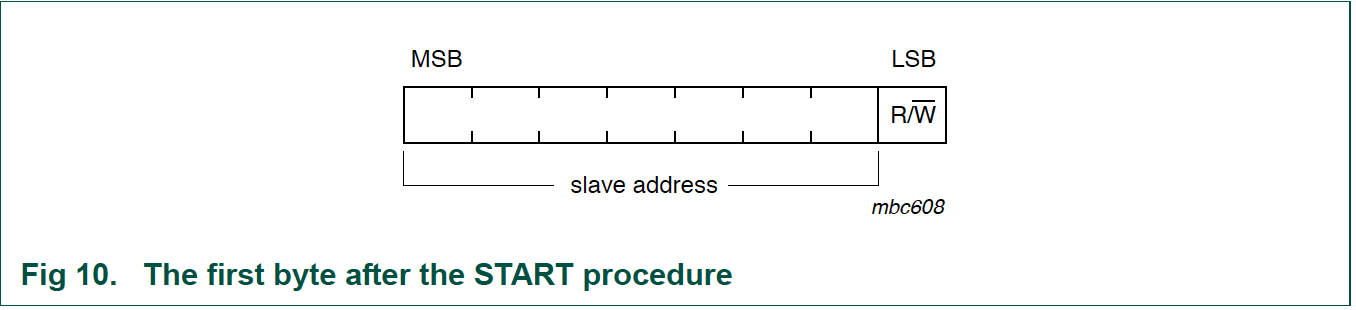
\includegraphics[scale=.65]{BilderAllgemein/I2C_slave_address.png}
  \caption{Erstes Byte nach Start Bedingung \ac{I$^2$C}  \citep[S. 13]{I2C_Datenblatt}}
  \label{Abb_Bild_I2C_Slave_Adresse}
\end{figure}

%Subsubsection Übertragungsprotokoll
\subsubsection*{Übertragungsprotokoll}
\label{subsubsection_Übertragungsprotokoll_I2C}
Das Übertragungsprotokoll beim \ac{I$^2$C} Bus ist immer so aufgebaut, dass die Kommunikation mit einem Start Signal beginnt und als nächstes das Byte mit der Slave Adresse und dem R\,/\,W Bit folgt. Jedes Byte das gesendet wird, wird durch den Slave mit einem ACK-Bit quittiert. Je nachdem wie das R\,/\,W Bit gesetzt ist (READ = 1, WRITE = 0) werden die Daten byteweise gelesen oder geschrieben. Das ACK Bit wird dann entweder vom Master oder vom Slave gesendet. Ist das letzte Byte der Übertragung gesendet, wird dieses vom Master mit einem NACK quittiert. Im Anschluss wird die Kommunikation durch die STOP Bedingung beendet. In Abbildung \ref{Abb_Bild_I2C_Slave_Adresse} ist der Ablauf noch einmal grafisch dargestellt.

%Grafik Übertragungsprotokoll
\begin{figure}[h!] 
  \centering
     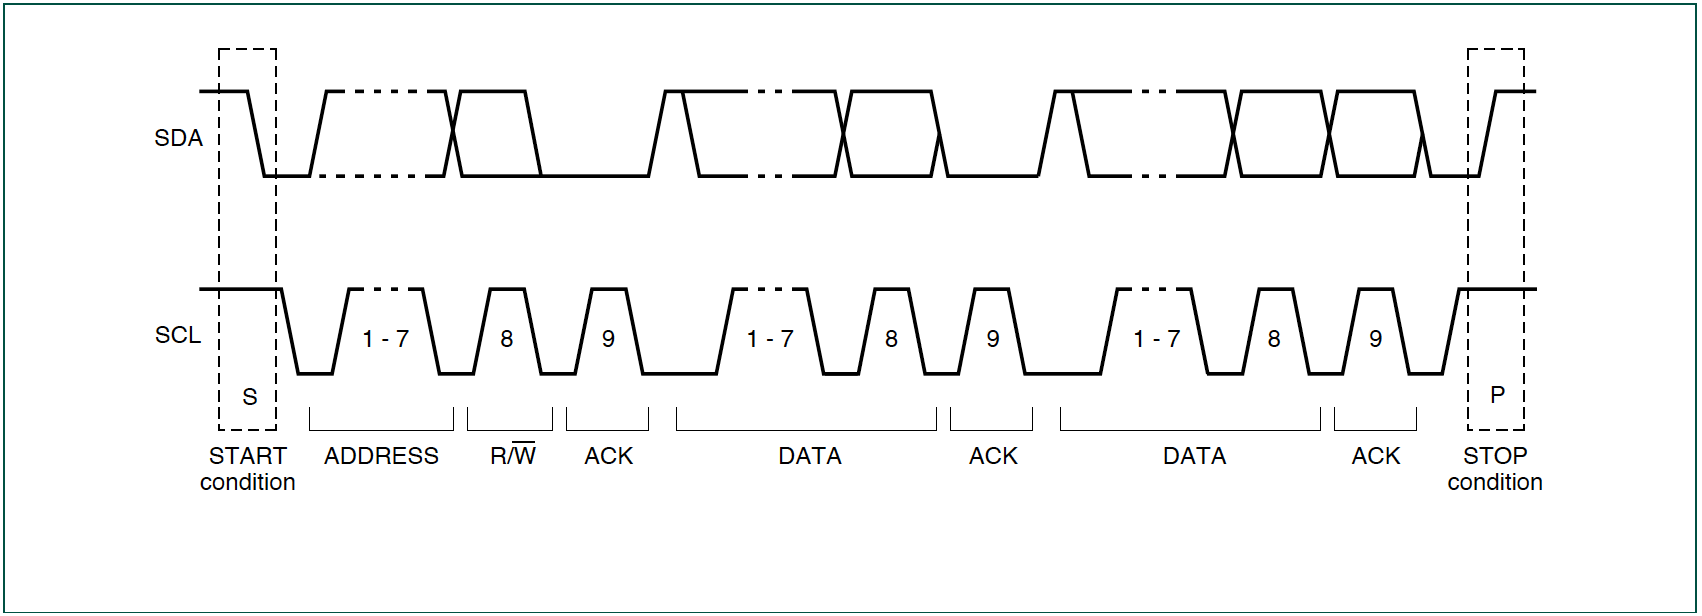
\includegraphics[scale=.53]{BilderAllgemein/I2C_data_transfer.png}
  \caption{Datentransfer \ac{I$^2$C} Bus  \citep[S. 13]{I2C_Datenblatt}}
  \label{Abb_Bild_I2C_Slave_Adresse}
\end{figure}
\newpage

